\documentclass[aspectratio=169,10pt]{beamer}

% Same look as the RP1 deck, so the two read as one project.
\usetheme{Madrid}
\useinnertheme{rounded}
\setbeamertemplate{blocks}[rounded][shadow=false]
\setbeamertemplate{navigation symbols}{}
\setbeameroption{hide notes}

\usepackage[T1]{fontenc}
\usepackage[utf8]{inputenc}
\usepackage{lmodern}
\usepackage{amsmath,amssymb}
\usepackage{booktabs}
\usepackage{array}
\usepackage{xcolor}
\usepackage{tikz}
\usetikzlibrary{positioning,arrows.meta,calc}
\usepackage{pgfplots}
\pgfplotsset{compat=1.18}

\definecolor{DeepBlue}{HTML}{0D1B2A}
\definecolor{MidBlue}{HTML}{1B4F72}
\definecolor{AccentBlue}{HTML}{2E86AB}
\definecolor{SoftBlue}{HTML}{EAF2F8}
\definecolor{WarmGold}{HTML}{E8A838}
\definecolor{SoftGold}{HTML}{FFF3CD}
\definecolor{MutedGray}{HTML}{4D5656}
\definecolor{Rust}{HTML}{B5523B}

\setbeamercolor{palette primary}{bg=DeepBlue,fg=white}
\setbeamercolor{palette secondary}{bg=MidBlue,fg=white}
\setbeamercolor{palette tertiary}{bg=AccentBlue,fg=white}
\setbeamercolor{structure}{fg=MidBlue}
\setbeamercolor{frametitle}{bg=SoftBlue,fg=MidBlue}
\setbeamercolor{block title}{bg=MidBlue!14,fg=MidBlue}
\setbeamercolor{block body}{bg=MidBlue!4,fg=black}
\setbeamercolor{block title alerted}{bg=WarmGold!90,fg=DeepBlue}
\setbeamercolor{block body alerted}{bg=SoftGold,fg=black}

\setbeamertemplate{footline}{%
  \leavevmode%
  \hbox{%
  \begin{beamercolorbox}[wd=.34\paperwidth,ht=3.2ex,dp=1.2ex,leftskip=0.8em]{palette primary}%
    \scriptsize\vphantom{Ag} Nour Gaser \& Mohamed Wael
  \end{beamercolorbox}%
  \begin{beamercolorbox}[wd=.48\paperwidth,ht=3.2ex,dp=1.2ex,center]{palette primary}%
    \scriptsize\vphantom{Ag} Research Project II
  \end{beamercolorbox}%
  \begin{beamercolorbox}[wd=.18\paperwidth,ht=3.2ex,dp=1.2ex,rightskip=0.8em]{palette secondary}%
    \hfill\scriptsize\vphantom{Ag} \insertframenumber/\inserttotalframenumber
  \end{beamercolorbox}}%
  \vskip0pt%
}

\setbeamersize{text margin left=0.6cm,text margin right=0.6cm}
\setbeamerfont{frametitle}{size=\large,series=\bfseries}
\setbeamerfont{block title}{size=\normalsize,series=\bfseries}
\setbeamerfont{block body}{size=\small}
\setbeamerfont{itemize/enumerate body}{size=\small}
\setbeamerfont{itemize/enumerate subbody}{size=\footnotesize}

\newcommand{\muted}[1]{\textcolor{MutedGray}{#1}}
\newcommand{\source}[1]{\vfill\hfill{\scriptsize\textcolor{MutedGray}{#1}}}

\title{Where the Signal Is}
\subtitle{Label provenance and the limits of fusion in Arabic multimodal affect recognition}
\author{Nour Gaser \and Mohamed Wael}
\institute{German International University}
\date{Research Project II, 2026}

\begin{document}

% ---------------------------------------------------------------- 1
{\setbeamertemplate{footline}{}
\setbeamercolor{background canvas}{bg=DeepBlue}
\begin{frame}[plain]
\vspace{1.2cm}
\begin{center}
{\color{white}\LARGE\bfseries Where the Signal Is}\\[0.3cm]
{\color{AccentBlue!30!white}\large Label provenance and the limits of fusion\\in Arabic multimodal affect recognition}\\[1.1cm]
{\color{white}\normalsize Nour Gaser \quad\&\quad Mohamed Wael}\\[0.15cm]
{\color{white!70}\small German International University \,\textperiodcentered\, Research Project II}
\end{center}
\note{Introduce ourselves. One sentence: in RP1 we proposed a cross-modal attention model for Egyptian Arabic emotion recognition; this is what happened when we built and tested it.}
\end{frame}
\setbeamercolor{background canvas}{bg=white}
}

% ---------------------------------------------------------------- 2
\begin{frame}[t]{What we set out to test (from RP1)}
\begin{columns}[T,onlytextwidth]
\column{0.52\linewidth}
In RP1 we proposed \textbf{Tri-CAN}: text features query the audio and video
features through cross-attention before classification.

\vspace{0.4cm}
The argument was that late fusion (encode each modality separately, concatenate
at the end) cannot catch cases where the words and the delivery disagree, such
as sarcasm.

\vspace{0.4cm}
\textbf{Question for RP2:} does cross-modal attention beat late fusion, and if
it does, is the advantage concentrated on samples where the modalities disagree?

\column{0.44\linewidth}
\begin{block}{Baseline to beat}
Gated late fusion on EGY-MER\\
weighted F1 = \textbf{0.519}\\
\muted{\footnotesize Hussein et al., 2025}
\end{block}
\begin{block}{Encoders}
\begin{tabular}{@{}ll@{}}
Text & AraBERT \\
Audio & wav2vec2 \\
Video & Swin / ViT \\
\end{tabular}
\end{block}
\end{columns}
\note{Keep this short, the committee knows RP1. The key sentence is the question at the bottom left: does attention help, and does it help most where the modalities disagree.}
\end{frame}

% ---------------------------------------------------------------- 3
\begin{frame}[t]{Two things changed after the proposal}
\begin{columns}[T,onlytextwidth]
\column{0.48\linewidth}
\begin{block}{EGY-MER arrived late}
We requested it and heard nothing back for months, so we built the pipeline on
\textbf{Ar-MuSA}, the one openly downloadable Arabic tri-modal corpus
(8,699 clips, 3-class sentiment).

\vspace{0.2cm}
EGY-MER arrived on 9 August. Everything was then repeated on it.
\end{block}
\column{0.48\linewidth}
\begin{block}{Part of the RP1 gap was closed by others}
Our systematic search (1,322 papers) found that cross-modal attention reached
Arabic \emph{sentiment} in 2026 (GCMA-Net and two related papers, all on Ar-MuSA).

\vspace{0.2cm}
It has still not been applied to Arabic \emph{emotion} recognition, which is
what EGY-MER is.
\end{block}
\end{columns}
\vspace{0.3cm}
\small Both changes pushed the project the same way: instead of just reporting
one more F1 score, we had to understand what these benchmarks can and cannot tell us.
\source{Ben Cheikhi et al., 2026; Khaled et al., 2025}
\note{Say plainly that the RP1 novelty claim was too broad and the updated RP1 report corrects it. Don't be defensive; finding this ourselves is part of doing the review properly.}
\end{frame}

% ---------------------------------------------------------------- 4
\begin{frame}[t]{How the experiments were run}
\begin{columns}[T,onlytextwidth]
\column{0.5\linewidth}
\begin{itemize}
\item Encoders are \textbf{frozen}; features are extracted once and cached.
      Only the fusion module and classifier are trained.
\item So when two models are compared, the fusion mechanism is the only thing that differs.
\item Stratified 5-fold cross-validation, \textbf{identical folds} for every model.
\item Predictions are collected out-of-fold, so every sample is predicted by a
      model that never trained on it.
\end{itemize}
\column{0.46\linewidth}
\begin{itemize}
\item EGY-MER results are the mean of \textbf{3 seeds}. A difference smaller
      than the seed standard deviation is treated as a tie.
\item Main metric: macro-F1 (the classes are very imbalanced).
      Weighted F1 only for comparing with the published baseline.
\item Controls: a late-fusion model widened to Tri-CAN's parameter count,
      and a synthetic corpus with no signal (the analysis must find nothing there).
\item Everything ran on CPU.
\end{itemize}
\end{columns}
\note{If asked why frozen: it makes the comparison cleaner, and we did fine-tune the text encoder later to check that the result holds (slide 11).}
\end{frame}

% ---------------------------------------------------------------- 5
\begin{frame}[t]{First result on Ar-MuSA: there was almost nothing to fuse}
\begin{columns}[T,onlytextwidth]
\column{0.5\linewidth}
\centering
\begin{tabular}{@{}lc@{}}
\toprule
Ar-MuSA, one seed & macro-F1 \\
\midrule
Text only   & 0.546 \\
Audio only  & 0.418 \\
Visual only & 0.433 \\
All three (late fusion) & 0.559 \\
\bottomrule
\end{tabular}

\vspace{0.4cm}
\raggedright
Adding audio and video to text gained only \textbf{+0.013}.
\column{0.46\linewidth}
Tri-CAN did not beat late fusion either, and neither did two other attention variants.

\vspace{0.3cm}
Before concluding that attention does not work, we checked whether the corpus
gives it any room to work in.
\end{columns}
\note{This was the point where we could have just written ``attention does not help''. Instead we asked why text alone is almost as good as everything together.}
\end{frame}

% ---------------------------------------------------------------- 6
\begin{frame}[t]{Label provenance: where does the label come from?}
Both corpora annotate each modality separately, plus an overall label.
So we can count how often a modality's own label equals the overall label.

\vspace{0.3cm}
\begin{columns}[T,onlytextwidth]
\column{0.5\linewidth}
\centering
\begin{tabular}{@{}lc@{}}
\toprule
Ar-MuSA annotation & agrees with overall \\
\midrule
Transcript & \textbf{96.5\%} \\
Audio      & 77.1\% \\
Frame      & 48.2\% \\
\bottomrule
\end{tabular}
\column{0.46\linewidth}
\begin{itemize}
\item Only 304 of 8,699 clips have an overall label different from the transcript label.
\item A model that perfectly predicted the transcript label would score
      macro-F1 \textbf{0.966} on the ``multimodal'' target.
\item The sarcasm flag behaves the same way (94.9\%).
\end{itemize}
\end{columns}
\vspace{0.4cm}
\small This is a property of the corpus. It applies to every published result on
Ar-MuSA, including the attention models, not only to ours.
\source{computed by \texttt{experiments/label\_provenance.py}}
\note{This is the central idea of the project, take your time. The overall label is basically the transcript label. So a text model already has almost all the information and no fusion method has room to show it is better.}
\end{frame}

% ---------------------------------------------------------------- 7
\begin{frame}[t]{The prediction, and what EGY-MER showed}
If label provenance is the problem, then a corpus whose label is \emph{not} in
the text should behave differently: non-verbal modalities should matter more,
and the gain from combining them should grow. We wrote this down before EGY-MER arrived.

\vspace{0.2cm}
\centering
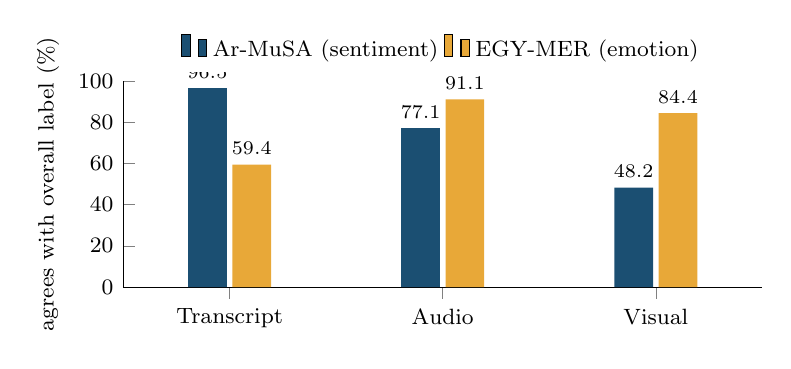
\begin{tikzpicture}
\begin{axis}[
  ybar, bar width=14pt, width=0.8\linewidth, height=4.2cm,
  ymin=0, ymax=100, ylabel={agrees with overall label (\%)},
  ylabel style={font=\footnotesize}, tick label style={font=\footnotesize},
  symbolic x coords={Transcript,Audio,Visual}, xtick=data,
  enlarge x limits=0.25, legend style={font=\footnotesize, at={(0.5,1.04)}, anchor=south, draw=none}, legend columns=2,
  nodes near coords, nodes near coords style={font=\scriptsize}, axis lines*=left,
]
\addplot[fill=MidBlue, draw=none] coordinates {(Transcript,96.5) (Audio,77.1) (Visual,48.2)};
\addplot[fill=WarmGold, draw=none] coordinates {(Transcript,59.4) (Audio,91.1) (Visual,84.4)};
\legend{Ar-MuSA (sentiment), EGY-MER (emotion)}
\end{axis}
\end{tikzpicture}

\raggedright\small
On EGY-MER the order flips: audio carries the label best, and 40.6\% of segments
have an overall label different from the transcript label.
\source{EGY-MER: 473 segments with all three modality labels}
\note{The bars flip. On Ar-MuSA the label lives in the words. On EGY-MER it lives in how things are said and shown.}
\end{frame}

% ---------------------------------------------------------------- 8
\begin{frame}[t]{The models behaved as predicted}
\begin{columns}[T,onlytextwidth]
\column{0.55\linewidth}
\centering
\begin{tabular}{@{}lcc@{}}
\toprule
macro-F1, one modality & Ar-MuSA & EGY-MER \\
\midrule
Text   & \textbf{0.546} & 0.340 \\
Audio  & 0.418 & 0.477 \\
Visual & 0.433 & \textbf{0.523} \\
\midrule
All three (late fusion) & 0.559 & 0.566 \\
Gain over best single   & +0.013 & \textbf{+0.044} \\
\bottomrule
\end{tabular}
\column{0.41\linewidth}
\begin{itemize}
\item Text goes from the best modality to the worst.
\item The benefit of using all three modalities is more than three times larger on EGY-MER.
\end{itemize}
\vspace{0.3cm}
So EGY-MER is a corpus where fusion \emph{can} be tested. The next question is
whether cross-modal attention does better than concatenation there.
\end{columns}
\source{base encoders, seed 0}
\note{The prediction from the previous slide holds in the model scores too, not just in the annotations.}
\end{frame}

% ---------------------------------------------------------------- 9
\begin{frame}[t]{Twelve fusion arrangements on EGY-MER}
\begin{columns}[T,onlytextwidth]
\column{0.6\linewidth}
\centering\scriptsize
\begin{tabular}{@{}lccr@{}}
\toprule
& \multicolumn{2}{c}{macro-F1, mean $\pm$ SD over 3 seeds} & \\
\cmidrule(lr){2-3}
arrangement & base encoders & best encoders & params \\
\midrule
late fusion (concatenation)   & \textbf{0.558} $\pm$ .006 & 0.594 $\pm$ .009 & 0.9M \\
late fusion, widened          & 0.553 $\pm$ .021 & 0.602 $\pm$ .012 & 1.9M \\
gated fusion (published)      & 0.530 $\pm$ .010 & 0.568 $\pm$ .015 & 1.1M \\
early fusion                  & 0.518 $\pm$ .010 & 0.571 $\pm$ .028 & 1.7M \\
all-pairs attention (MulT)    & 0.535 $\pm$ .021 & 0.574 $\pm$ .019 & 6.4M \\
Tri-CAN, text anchor          & 0.548 $\pm$ .011 & 0.559 $\pm$ .004 & 1.9M \\
Tri-CAN, audio anchor         & 0.514 $\pm$ .005 & 0.544 $\pm$ .010 & 1.9M \\
Tri-CAN, visual anchor        & 0.539 $\pm$ .017 & 0.554 $\pm$ .015 & 1.9M \\
hybrid, text anchor           & 0.541 $\pm$ .005 & 0.583 $\pm$ .013 & 2.5M \\
hybrid, audio anchor          & 0.544 $\pm$ .007 & 0.570 $\pm$ .024 & 2.5M \\
hybrid, visual anchor         & 0.545 $\pm$ .005 & 0.559 $\pm$ .014 & 2.5M \\
hybrid + gate, text anchor    & 0.557 $\pm$ .014 & \textbf{0.608} $\pm$ .017 & 2.7M \\
\bottomrule
\end{tabular}
\column{0.36\linewidth}
\small
\begin{itemize}
\item No arrangement beats plain concatenation by more than the seed spread,
      with either set of encoders.
\item Concatenation is also the smallest model.
\item The three Tri-CAN variants are in the bottom half both times.
\item Anchoring on audio or video, EGY-MER's stronger modalities, did not help.
\end{itemize}
\end{columns}
\source{best encoders: AraBERT-twitter, wav2vec2 mid-layer, face-expression ViT}
\note{Be careful with wording here. With the best encoders, hybrid+gate is 0.608 against 0.594, but the seed SD is 0.017, so it's a tie, not a win. What we can say: nothing beats concatenation beyond noise, and Tri-CAN itself is never near the top.}
\end{frame}

% ---------------------------------------------------------------- 10
\begin{frame}[t]{Why Tri-CAN loses: a flaw in our own design}
\begin{columns}[T,onlytextwidth]
\column{0.53\linewidth}
\centering
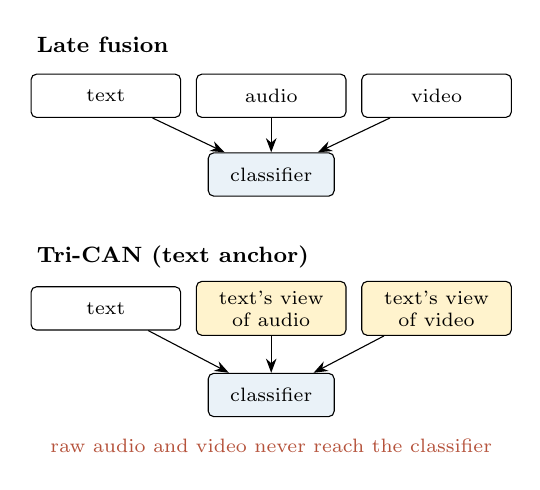
\begin{tikzpicture}[font=\scriptsize, >={Stealth[length=1.8mm]},
  box/.style={draw, rounded corners=2pt, minimum width=1.9cm, minimum height=0.55cm, align=center},
  clf/.style={draw, rounded corners=2pt, fill=SoftBlue, minimum width=1.6cm, minimum height=0.55cm}]
\node[font=\footnotesize\bfseries, anchor=west] at (-0.2,2.75) {Late fusion};
\node[box] (t1) at (0.8,2.1) {text};
\node[box] (a1) at (2.9,2.1) {audio};
\node[box] (v1) at (5.0,2.1) {video};
\node[clf] (c1) at (2.9,1.1) {classifier};
\draw[->] (t1) -- (c1); \draw[->] (a1) -- (c1); \draw[->] (v1) -- (c1);

\node[font=\footnotesize\bfseries, anchor=west] at (-0.2,0.05) {Tri-CAN (text anchor)};
\node[box] (t2) at (0.8,-0.6) {text};
\node[box, fill=SoftGold] (a2) at (2.9,-0.6) {text's view\\of audio};
\node[box, fill=SoftGold] (v2) at (5.0,-0.6) {text's view\\of video};
\node[clf] (c2) at (2.9,-1.7) {classifier};
\draw[->] (t2) -- (c2); \draw[->] (a2) -- (c2); \draw[->] (v2) -- (c2);
\node[text=Rust, align=center] at (2.9,-2.35) {raw audio and video never reach the classifier};
\end{tikzpicture}
\column{0.43\linewidth}
\small
All three inputs to Tri-CAN's classifier are pooled over the \emph{text} positions.
So Tri-CAN does not add attention on top of late fusion; it replaces audio and
video with what text finds in them, and has less information than the baseline.

\vspace{0.25cm}
On incongruent samples every anchor scores below late fusion
($-0.047$, $-0.070$, $-0.066$).

\vspace{0.25cm}
\textbf{Repair:} the ``hybrid'' models give the classifier the raw vectors too.
With a gate added, text-anchored attention goes from $-0.010$ to $-0.001$
behind late fusion: a tie, not a gain.
\end{columns}
\note{We found this ourselves by looking at where Tri-CAN loses. The congruent vs incongruent difference is consistent in direction, but its bootstrap 95\% interval is [-0.19, +0.03] and includes zero, so present it as a direction, not a proven effect. The hybrid repair confirms the diagnosis but shows the attended view adds nothing new.}
\end{frame}

% ---------------------------------------------------------------- 11
\begin{frame}[t]{Where the improvements actually came from}
\centering
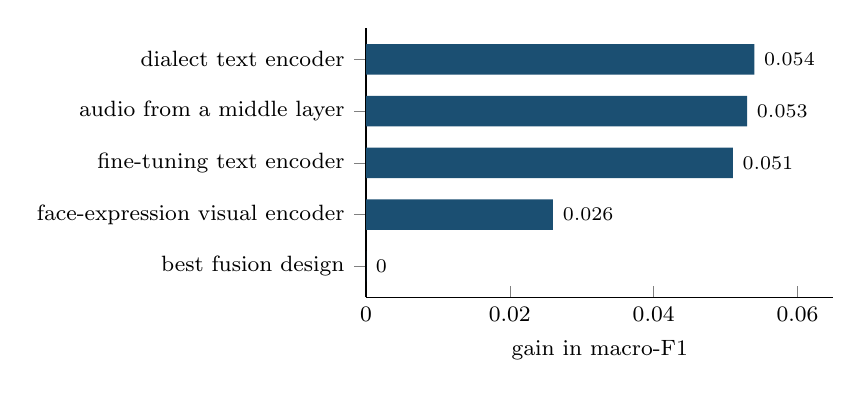
\begin{tikzpicture}
\begin{axis}[
  xbar, bar width=11pt, width=0.62\linewidth, height=5.0cm,
  xmin=0, xmax=0.065, xlabel={gain in macro-F1}, xlabel style={font=\footnotesize},
  scaled x ticks=false, xticklabel style={/pgf/number format/fixed, /pgf/number format/precision=2},
  tick label style={font=\footnotesize},
  symbolic y coords={best fusion design,face-expression visual encoder,fine-tuning text encoder,audio from a middle layer,dialect text encoder},
  ytick=data, enlarge y limits=0.15, axis lines*=left,
  nodes near coords, nodes near coords style={font=\scriptsize, /pgf/number format/fixed, /pgf/number format/precision=3},
]
\addplot[fill=MidBlue, draw=none] coordinates {(0.054,dialect text encoder) (0.053,audio from a middle layer) (0.051,fine-tuning text encoder) (0.026,face-expression visual encoder) (0,best fusion design)};
\end{axis}
\end{tikzpicture}

\raggedright\small
\begin{itemize}
\item Dialect text encoder: AraBERT-twitter instead of the MSA-trained AraBERTv2 (Ar-MuSA).
\item Audio: the last wav2vec2 layer is tuned to its pretraining task; layer 10 carries more prosody (EGY-MER).
\item Fine-tuning the text encoder raised late fusion and Tri-CAN by the same $+0.050$, so their order did not change.
\end{itemize}
\note{Every real gain came from better representations, not from the fusion architecture. The fine-tuning point matters: it shows the fusion result is not just an artefact of frozen encoders.}
\end{frame}

% ---------------------------------------------------------------- 12
\begin{frame}[t]{Hypotheses we tested and had to reject}
\begin{enumerate}
\item \textbf{Anchor choice.} Text is EGY-MER's weakest modality, so anchoring on
      audio or video should help. It did not (audio $-0.034$, video $-0.009$ against text).
\item \textbf{Multilingual audio encoder.} XLS-R scored lower than English
      wav2vec2-base on Ar-MuSA (0.384 vs 0.421). The weak audio was not a language mismatch.
\item \textbf{Face cropping.} Cropping to the largest detected face lowered
      macro-F1 by 0.038, although faces were found in 98\% of frames. In talk-show
      footage the largest face is often not the person speaking.
\item \textbf{Emotion-trained audio encoder.} A wav2vec2 fine-tuned for English
      acted emotion scored lower than the generic one (0.458 vs 0.477).
\end{enumerate}
\vspace{0.3cm}
\small From 2 and 4: matching the encoder's language and domain to the data helped;
matching its training labels to our task did not.
\note{We wrote each of these down before running it. Reporting the ones that failed is part of the result, and it answers ``did you try X'' questions before they come.}
\end{frame}

% ---------------------------------------------------------------- 13
\begin{frame}[t]{Comparison with the published EGY-MER baseline}
\begin{columns}[T,onlytextwidth]
\column{0.5\linewidth}
\centering
\begin{tabular}{@{}lc@{}}
\toprule
& weighted F1 \\
\midrule
Hussein et al. (gated late fusion) & 0.519 \\
Ours, late fusion, base encoders & 0.654 \\
Ours, late fusion, best encoders & \textbf{0.669} \\
\bottomrule
\end{tabular}
\\[0.15cm]
{\scriptsize\muted{ours: mean of 3 seeds, 5-fold CV}}
\column{0.46\linewidth}
\begin{alertblock}{Not a like-for-like comparison}
The published result uses 363 samples and its own splits.
The corpus we received has 505 annotated segments; we use the 484 labelled with
one of the seven emotions.
\end{alertblock}
\end{columns}
\vspace{0.3cm}
\small We report it because it is the only published number on this corpus, but the
contribution of this project is the analysis, not this score.
\note{If asked: the RP2 report quotes 0.664, which is the single-seed run of the base model. The 3-seed mean is 0.654. Both are well above 0.519, and neither is directly comparable.}
\end{frame}

% ---------------------------------------------------------------- 14
\begin{frame}[t]{Limitations}
\begin{itemize}
\item \textbf{Small corpus.} 484 samples over 7 classes, with only 12 Fear and 18
      Happiness. Macro-F1 is noisy, which is why we use seeds and call small differences ties.
\item \textbf{Frozen audio and video encoders.} Only the text encoder was fine-tuned;
      doing the others needs a GPU we did not have.
\item \textbf{Annotations are a proxy.} ``The modalities disagree'' means the annotators
      labelled them differently, not that we measured the signal directly.
\item \textbf{No grouping by source video.} Folds are stratified by label but the same
      speaker can appear in train and test. This affects absolute scores more than the
      comparisons, since every model uses the same folds.
\item \textbf{The corpus we received differs from the paper's} (505 annotated segments vs 363).
\end{itemize}
\note{Say these before being asked. Each one is also written in the report.}
\end{frame}

% ---------------------------------------------------------------- 15
\begin{frame}[t]{Conclusion}
\begin{enumerate}
\item On Ar-MuSA, the overall label matches the transcript annotation 96.5\% of the time.
      That leaves no room to compare fusion methods on it. This is cheap to measure
      and we think it should be reported with any multimodal benchmark.
\item On EGY-MER, where the label is mostly in audio and video, fusion does matter,
      but plain concatenation was as good as any attention design we tried.
\item The gains we did get came from choosing and using encoders well.
\end{enumerate}

\vspace{0.4cm}
\begin{block}{Next steps}
\begin{itemize}
\item Measure label provenance on MORAD (same 7 emotions, about 6$\times$ larger).
\item Active-speaker detection, so that face-based features look at the right person.
\item Folds grouped by source video.
\end{itemize}
\end{block}
\note{Three points. If time is short, say only the first sentence of each.}
\end{frame}

% ---------------------------------------------------------------- 16
{\setbeamertemplate{footline}{}
\setbeamercolor{background canvas}{bg=DeepBlue}
\begin{frame}[plain]
\vspace{2.2cm}
\begin{center}
{\color{white}\LARGE Thank you}\\[0.4cm]
{\color{white!70}\normalsize Code, results and reports: \href{https://github.com/nourgaser/giu-ms-rp}{\texttt{github.com/nourgaser/giu-ms-rp}}}
\end{center}
\end{frame}
\setbeamercolor{background canvas}{bg=white}
}

% ---------------------------------------------------------------- backup
\appendix
\begin{frame}[t]{Backup: controls behind the null result}
\begin{itemize}
\item \textbf{Capacity-matched baseline.} Late fusion widened to Tri-CAN's parameter
      count (1.9M). It does not overtake the plain version beyond seed noise,
      so ``Tri-CAN lost because it is bigger or smaller'' is ruled out.
\item \textbf{Null corpus.} On synthetic data with no signal, the analysis gives chance-level
      scores and a difference-in-differences interval containing zero (2 automated tests).
\item \textbf{Out-of-fold predictions.} Subgroup results (congruent, incongruent) are
      computed on predictions from models that never saw those samples.
\item \textbf{Same folds, features and training loop} for every model compared.
\end{itemize}
\vspace{0.3cm}
\small Congruent vs incongruent, text-anchored Tri-CAN minus late fusion:
$+0.036$ and $-0.046$; difference $-0.082$, 95\% bootstrap interval $[-0.189, +0.034]$
(208 and 265 samples). The direction is consistent; the interval includes zero.
\end{frame}

\end{document}
